\section{Variables aleatorias y distribuciones de probabilidad}

\paragraph{Finalidad :} Abstraer matemáticamente un tipo de experimento aleatorio. Y, con ello, poder estimar de manera teórica lo que sucedería de manera experimental mediante una estadística. 

\paragraph{¿Cómo?:} Mediante variables aleatorias y distribuciones de probabilidad asociadas a esas variables:

\section{Variables aleatorias} Una variable aleatoria es una función que a cada suceso
elemental de un espacio muestral le asigna un número. Para hacer referencia a las variables se usan las letras: $X$, $Y$, ...

\paragraph{Ejemplo:} Sea el experimento aleatorio “lanzar un dado”: El espacio muestral lo componen las 6 caras del dado. Podemos asignar la variable $X$ que a cada cara le asocia el número que represente su cara.

\begin{center}
\begin{tabular}{ccc}
 & $X$ &  \\
Suceso &  &  $x_i$\\ \hline 
Cara 1 & $\rightarrow$ & 1 \\ 
Cara 2 & $\rightarrow$ & 2 \\ 
Cara 3 & $\rightarrow$ & 3 \\ 
Cara 4 & $\rightarrow$ & 4 \\ 
Cara 5 & $\rightarrow$ & 5 \\ 
Cara 6 & $\rightarrow$ & 6 \\ 
\end{tabular} 
\end{center}

\paragraph{Ejemplo:} Sea el experimento compuesto lanzar dos monedas. Podemos asignar la variable aleatoria: $$Y=\left\lbrace Número \ de \ caras \right\rbrace$$

\begin{center}
\begin{tabular}{ccc}
 & $Y$ &  \\
Suceso &  &  $y_i$\\ \hline 
C,C & $\rightarrow$ & 2 \\ 
C,X & $\rightarrow$ & 1 \\ 
X,C & $\rightarrow$ & 1 \\ 
X,X & $\rightarrow$ & 0 \\ 
\end{tabular} 
\end{center}

\subsection{Tipos de variables aleatorias}
\begin{description}
\item[Discretas:] Toman un número finito o numerable de valores
\item[Continuas:] Toman valores en un rango continuo
\end{description}

\paragraph{Ejemplo de variables discreta:} Sea la \emph{X =“El número de caras al lanzar dos dados”}. Los valores posibles son 0, 1 o 2 (que es un conjunto finito de datos, en concreto 3 datos) 

\paragraph{Ejemplo de variables continua:} \emph{X = “Distancia al centro de la diana medida desde la posición en que cae un dardo lanzado por un tirador experto” }. En este caso la variable puede tomar cualquier valor en el rango entre 0 y el radio de la diana 

\section{Distribuciones de probabilidad}

Llamaremos Distribución de probabilidad a la relación entre los valores de la variable y sus probabilidades.

Estas relaciones se pueden indicar mediante el uso de funciones. El tipo de función y su tratamiento es diferente según las variables sean discretas o continuas.

Veamos algunas distribuciones:


\section{Distribución uniforme discreta}

\paragraph{Ejemplo: } Sea la variable \emph{X = “Número obtenido al lanzar una dado”}\\
A cada valor de la variable podemos asignarle su probabilidad:

%\begin{center}
%\begin{tabular}{ccc}
% & $P(X)$ &  \\
%Suceso &  &  $y_i$ \\ \hline 
%1 & $\rightarrow$ & \frac{1}{6} \\ 
%2 & $\rightarrow$ & \frac{1}{6} \\ 
%3 & $\rightarrow$ & \frac{1}{6} \\ 
%4 & $\rightarrow$ & \frac{1}{6} \\ 
%5 & $\rightarrow$ & \frac{1}{6} \\ 
%6 & $\rightarrow$ & \frac{1}{6} \\ 
%\end{tabular} 
%\end{center}

\begin{center}
\begin{tabular}{ccc}
 & $P(X)$ &  \\
$x_i$ &  &  $P(x_i)$\\ \hline 
1 & $\rightarrow$ & $\tfrac{1}{6}$ \\ 
2 & $\rightarrow$ & $\tfrac{1}{6}$ \\ 
3 & $\rightarrow$ & $\tfrac{1}{6}$ \\ 
4 & $\rightarrow$ & $\tfrac{1}{6}$ \\ 
5 & $\rightarrow$ & $\tfrac{1}{6}$ \\ 
6 & $\rightarrow$ & $\tfrac{1}{6}$ \\ 
\end{tabular} 
\end{center}

Podemos representar la relación anterior mediante una función:

%$$f\colon \begin{array}{lc} 
%         & X \rightarrow Y \\ 
%         & x \mapsto f(x)=\frac{x-1}{2} 
%         \end{array}$$
%
%
%$$f\colon \begin{array}{>{\displaystyle}l} 
%          X \rightarrow Y \\ 
%          x\mapsto f(x)=\frac{x-1}{2} 
%         \end{array}$$

$$P\colon \begin{array}{ll} 
          X \rightarrow \mathbb{R} \\ 
          x_i\mapsto P(X=x_i)=\frac{1}{n} 
         \end{array}$$

Todas las caras tienen la misma probabilidad: $\frac{1}{n}$, siendo $n$ el número de caras, o tamaño del espacio muestral. 

A este tipo de distribución se le llama \textbf{uniforme discreta}.

\section{Distribución Binomial}

\paragraph{Ejemplo:} Queremos calcular las probabilidades de que al lanzar 5 monedas, obtengamos tres caras.
Un suceso que cumple el enunciado es:
$$S_1=\left\lbrace C,C,C,X,X \right\rbrace$$
Teniendo en cuenta que lanzar cada moneda son experimentos independientes, la probabilidad de ese suceso será:
%$$P\left(S_1\right)=P\left(C_1\right)\cdot P\left(C_2 C_1 \right)$$
\begin{eqnarray*}
P\left(S_1\right) & = &P\left(C_1\right)\cdot P\left(C_2 | C_1 \right)\cdot ... \cdot P\left(X_5 | C_1 \cap C_2  \cap C_3  \cap X_4   \right)= \\ &  = & P\left(C_1\right)\cdot  P\left(C_2\right) \cdot P\left(C_3\right) \cdot P\left(X_4\right) \cdot P\left(X_5\right)= \\
& = & P\left(C\right)^3\cdot  P\left(X\right)^2
\end{eqnarray*}

Como la probabilidad de que una moneda sea cara es $\frac{1}{2}$ y la de que sea cruz también:

$$P\left(S_1\right)=\left(\frac{1}{2}\right)^3\cdot  \left(\frac{1}{2}\right)^2$$

Ahora bien, habrá tantos sucesos que cumplan el enunciado como combinaciones de 5 elementos tomados de 3 en 3. Por tanto la probabilidad de que salgan 3 caras será:

$$P\left(Salgan \ 3 \ caras\right)=\binom{5}{3}\left(\frac{1}{2}\right)^3\cdot  \left(\frac{1}{2}\right)^2$$

Si asociamos al experimento "lanzar 5 monedas" le asignamos la variable "número de caras obtenidas", podemos determinar la probabilidad mediante la siguiente función.

$$P\colon \begin{array}{l} 
          X \rightarrow \mathbb{R} \\ 
          k\mapsto P(X=k)=\binom{5}{k}\left(\frac{1}{2}\right)^k\cdot  \left(\frac{1}{2}\right)^{5-k} 
         \end{array}$$

Esto es un ejemplo de distribución binomial de tamaño $5$ y probabilidad $0.5$ .

Realizando los cálculos para $k = 1,...,5 $, la distribución de probabilidad de $X$ que resulta es:

\begin{center}
\begin{tabular}{ccc}
 & $P(X)$ &  \\
$x_i$ &  &  $P(x_i)$\\ \hline 
0 & $\rightarrow$ & $0.03125$ \\ 
1 & $\rightarrow$ & $0.15625$ \\ 
2 & $\rightarrow$ & $0.3125$ \\ 
3 & $\rightarrow$ & $0.3125$ \\ 
4 & $\rightarrow$ & $0.15625$ \\ 
5 & $\rightarrow$ & $0.03125$ \\ 
\end{tabular} 
\end{center}

Y gráficamente: 

%\documentclass{article}
%\usepackage{pgfplots}
%\pgfplotsset{compat=1.7}
%
%\begin{document}
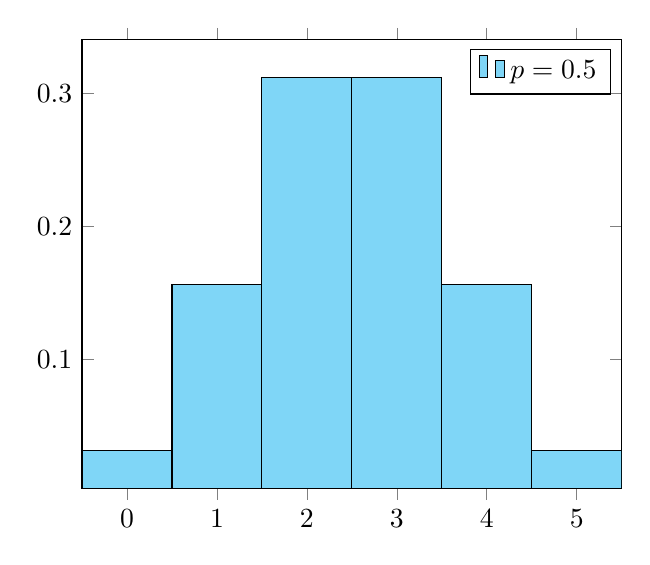
\begin{tikzpicture}[
    declare function={binom(\k,\n,\p)=\n!/(\k!*(\n-\k)!)*\p^\k*(1-\p)^(\n-\k);}
]
\begin{axis}[
    samples at={0,...,5},
    yticklabel style={
        /pgf/number format/fixed,
        /pgf/number format/fixed zerofill,
        /pgf/number format/precision=1
    },
    ybar=0pt, bar width=1
]
\addplot [fill=cyan, fill opacity=0.5] {binom(x,5,0.5)}; \addlegendentry{$p=0.5$}

\end{axis}
\end{tikzpicture}
%\end{document}


\paragraph{Generalización de distribución Binomial:} Hablaremos de una distribución binomial cuando:
\begin{itemize}
\item Se parte de un experimento compuesto de varios simples independientes
\item Los experimentos simples son dicotómicos. Es decir, solo puede haber dos sucesos elementales: uno al que llamaremos acierto y otro al que llamaremos fracaso
\item Asociado al experimento compuesto tenemos la variable número de aciertos cuando realizamos el experimento simple un número determinado de veces
\end{itemize}

En la situación anterior, la distribución binomial vendrá determinada por dos parámetros:
\begin{itemize}
\item Parámetro $n$: Número de veces que se realiza el experimento simple 
\item Parámetro $p$: La probabilidad de que ocurra el suceso acierto
\end{itemize}


A este tipo de variable y su distribución de probabilidades se le llama binomial. \\


\paragraph{Ejemplo:} Así en el ejemplo de las monedas, el experimento se compone de \textbf{5 lanzamientos de moneda}. Si sale cara es acierto y si no fracaso. La variable aleatoria asociada al experimento será el número de caras que salen al lanzar 5 monedas. Esta variable sigue una distribución binomial.

\subsection{Probabilidad de la binomial}\textbf{En general tendremos una binomial de tamaño $n$ y probabilidad $p$}, cuando el experimento simple se haga $n$ veces y la probabilidad de acierto sea $p$.

La función de probabilidad en este caso nos queda:
 
 $$P\colon \begin{array}{l} 
          X \rightarrow \mathbb{R} \\ 
          k\mapsto P(X=k)=\binom{n}{k}\left(p\right)^k\cdot  \left(1-p\right)^{n-k} 
         \end{array}$$
         
\paragraph{Ejemplos:} Representación gráfica de algunas binomiales:    
         
%\documentclass{article}
%\usepackage{pgfplots}
%
%\begin{document}
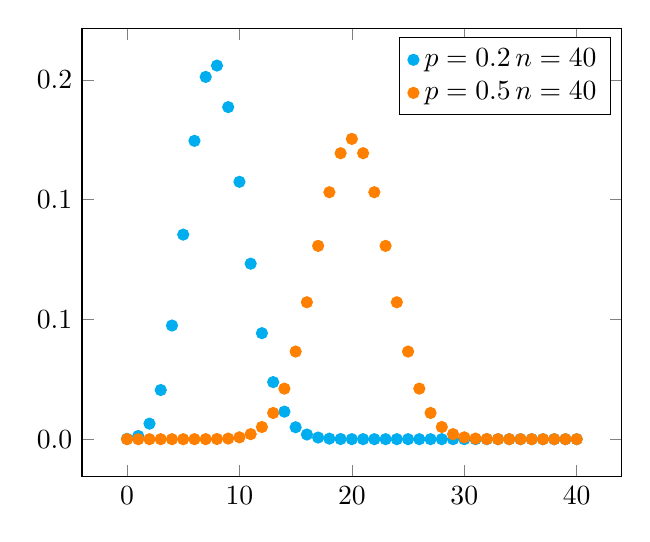
\begin{tikzpicture}[
    declare function={binom(\k,\n,\p)=\n!/(\k!*(\n-\k)!)*\p^\k*(1-\p)^(\n-\k);}
]
\begin{axis}[
    samples at={0,...,40},
    yticklabel style={
        /pgf/number format/fixed,
        /pgf/number format/fixed zerofill,
        /pgf/number format/precision=1
    }
]
\addplot [only marks, cyan] {binom(x,40,0.2)}; \addlegendentry{$p=0.2 \, n=40$}
\addplot [only marks, orange] {binom(x,40,0.5)}; \addlegendentry{$p=0.5 \, n=40 $}
\end{axis}
\end{tikzpicture}
%\end{document}
         
 

\section{Distribución Normal}
Se trata de una distribución asociada a a un variable continua. Tiene dos parámetros:
\begin{itemize}
    \item $\mu :$ Media de la distribución
    \item $\sigma :$ Desviación típica
\end{itemize}
Y se denota así: $
X \sim \mathcal{N}(\mu,\,\sigma)\,.
    $ 
    
La probabilidad total es 1 y la variable $X$ puede tomar $\infty$ valores ($x \in \left(-\infty, +\infty\right)$). Por tanto, en variables continuas la probabilidad de que tome un valor concreto será 0 ($\lim_{x \to \infty}\frac{1}{x}=0$).    

\subsection{función de densidad de una variable continua:}  En variables continuas solo tiene sentido calcular la probabilidad en intervalos.
Se llama \textbf{función de densidad} ($f(x)$) aquella que: 

$$P\left(a\leq X \leq b \right) = \int_{a}^{b} f(x) dx$$

La interpretación gráfica de lo anterior nos dice que la probabilidad de un intervalo corresponde con el área de la función de densidad en ese intervalo.

%\documentclass{article}
%\usepackage{pgfplots}
%\usetikzlibrary{math}
%\begin{document}



\begin{tikzpicture}[scale=0.7]

\pgfmathdeclarefunction{gauss}{2}{%
  \pgfmathparse{1/(#2*sqrt(2*pi))*exp(-((x-#1)^2)/(2*#2^2))}%
}

\tikzmath{
			\conf = 0.96; \crit= 2.05; \a=round(1-\conf)/2,2);
          }

%\begin{axis}[
%  no markers, domain=0:10, samples=100,
%  axis lines*=left, xlabel=$x$, ylabel=$y$,
%  every axis y label/.style={at=(current axis.above origin),anchor=south},
%  every axis x label/.style={at=(current axis.right of origin),anchor=west},
%  height=5cm, width=12cm,
%  xtick={4,6.5}, ytick=\empty,
%  enlargelimits=false, clip=false, axis on top,
%  grid = major
%  ]
%  \addplot [fill=cyan!20, draw=none, domain=0:5.96] {gauss(6.5,1)} \closedcycle;
%  \addplot [very thick,cyan!50!black] {gauss(4,1)};
%  \addplot [very thick,cyan!50!black] {gauss(6.5,1)};
%
%
%%\draw [yshift=-0.6cm, latex-latex](axis cs:4,0) -- node [fill=white] {$1.96\sigma$} (axis cs:5.96,0);
%\end{axis}

\begin{axis}[
  no markers, domain=-5:5, samples=100,
  axis lines=left, 
  %xlabel=$xa$, ylabel=$ya$,
  %every axis y label/.style={at=(current axis.above origin),anchor=south},
  %every axis x label/.style={at=(current axis.right of origin),anchor=west},
  height=5cm, width=12cm,
  xtick={-1,\crit}, ytick=\empty,
  xticklabels = {$a$, $b$},
  enlargelimits=false, clip=false, axis on top,
  %grid = major
  ]
  \addplot [fill=cyan!20, draw=none, domain=-1:\crit] {gauss(0,1)} \closedcycle;
  \addplot [very thick,cyan!50!black] {gauss(0,1)};
  %\addplot [very thick,cyan!50!black] {gauss(6.5,1)};
  


%\draw [yshift=-0.6cm, latex-latex](axis cs:4,0) -- node [fill=white] {$1.96\sigma$} (axis cs:5.96,0);
\end{axis}
\node[] at (5.5,1.5) {$P\left(a\leq X \leq b \right) $};	




\end{tikzpicture}

%\end{document}

\subsection{función de densidad de una distribución normal:}  En el caso de una $
X \sim \mathcal{N}(\mu,\,\sigma)
    $, la función de densidad es:
    $$f(x)=\frac{1}{{\sigma \sqrt {2\pi } }}e^{{{ - \left( {x - \mu } \right)^2 } \mathord{\left/ {\vphantom {{ - \left( {x - \mu } \right)^2 } {2\sigma ^2 }}} \right. \kern-\nulldelimiterspace} {2\sigma ^2 }}}$$
\paragraph{Ejemplos de representaciones gráficas de normales:} 
%\documentclass{article}
%\usepackage{pgfplots}
%\begin{document}



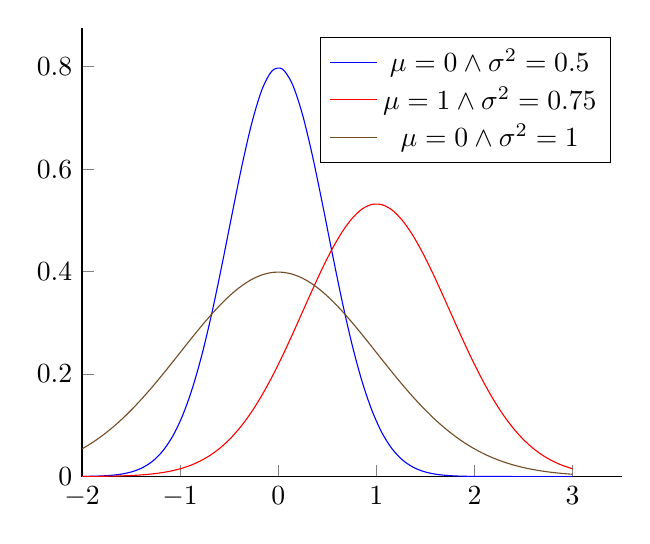
\begin{tikzpicture}
\pgfmathdeclarefunction{gauss}{2}{%
  \pgfmathparse{1/(#2*sqrt(2*pi))*exp(-((x-#1)^2)/(2*#2^2))}%
}

\begin{axis}[every axis plot post/.append style={
  mark=none,domain=-2:3,samples=50,smooth}, % All plots: from -2:2, 50 samples, smooth, no marks
  axis x line*=bottom, % no box around the plot, only x and y axis
  axis y line*=left, % the * suppresses the arrow tips
  enlargelimits=upper] % extend the axes a bit to the right and top
  \addplot {gauss(0,0.5)};
  \addlegendentry{$\mu=0 \land \sigma^{2}=0.5$}
  \addplot {gauss(1,0.75)};
  \addlegendentry{$\mu=1 \land \sigma^{2}=0.75$}
  \addplot {gauss(0,1)};
  \addlegendentry{$\mu=0 \land \sigma^{2}=1$}
\end{axis}
\end{tikzpicture}


%\end{document}

\subsection{Cálculo práctico de la probabilidad de la Normal:} En realidad, para calcular la probabilidad no se hace la integral, sino que se utiliza una tabla que ya tiene calculadas probabilidades de la  $Z \sim \mathcal{N}(0,\,1)\,.
    $.
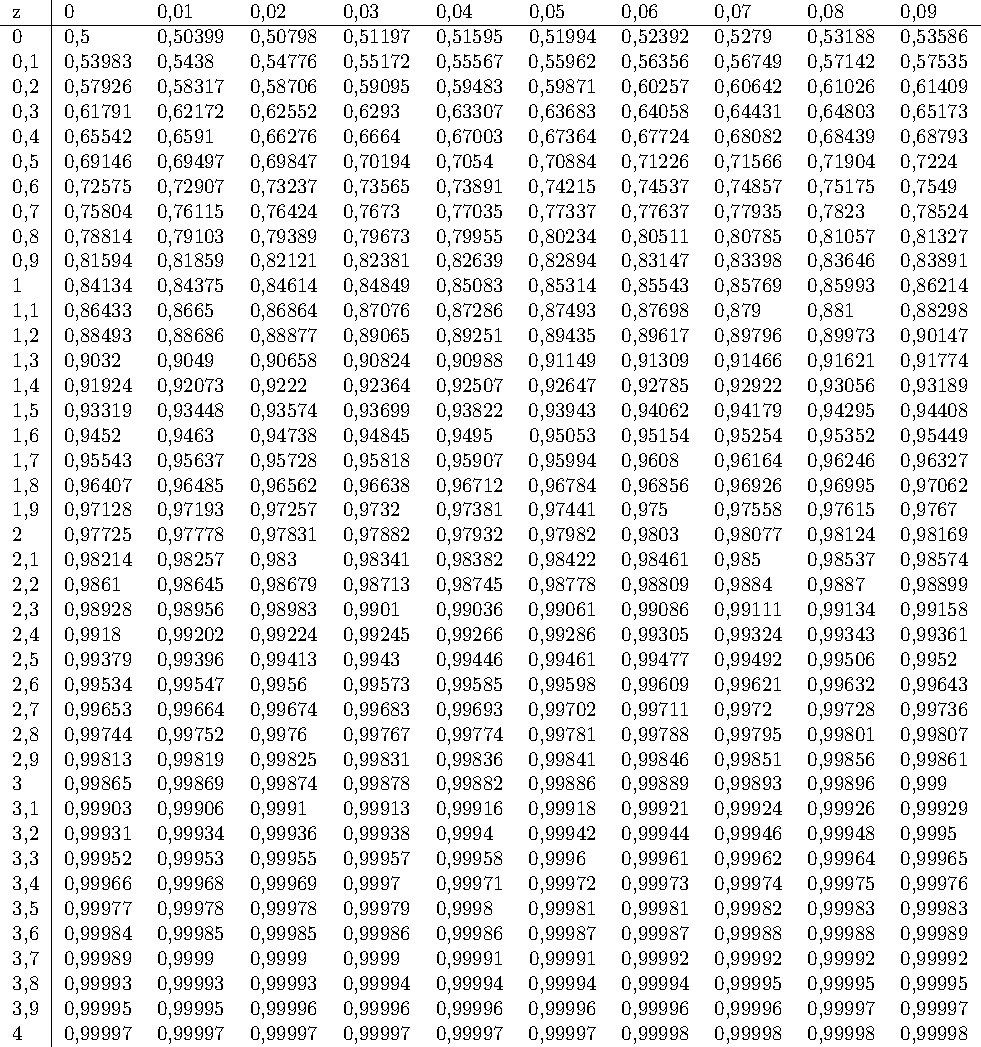
\includepdf[pages=-, scale=0.9]{distribucion_normal.pdf}

%\documentclass{article}
%\usepackage{pgfplots}
%\begin{document}



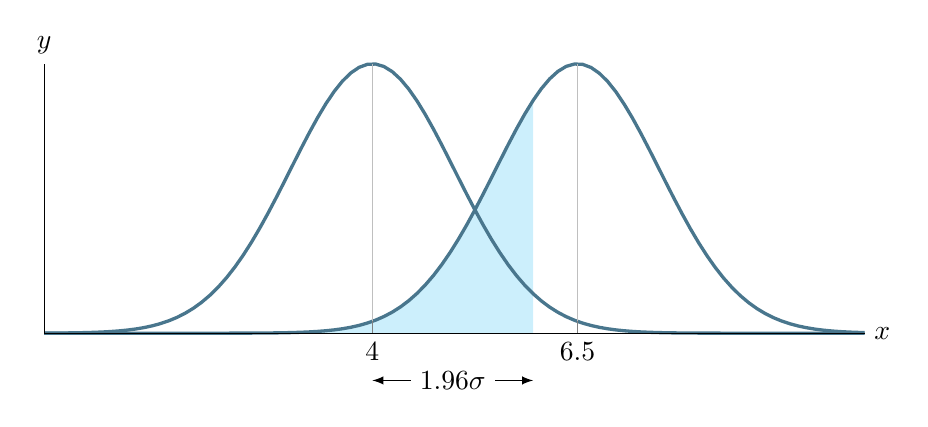
\begin{tikzpicture}

\pgfmathdeclarefunction{gauss}{2}{%
  \pgfmathparse{1/(#2*sqrt(2*pi))*exp(-((x-#1)^2)/(2*#2^2))}%
}

\begin{axis}[
  no markers, domain=0:10, samples=100,
  axis lines*=left, xlabel=$x$, ylabel=$y$,
  every axis y label/.style={at=(current axis.above origin),anchor=south},
  every axis x label/.style={at=(current axis.right of origin),anchor=west},
  height=5cm, width=12cm,
  xtick={4,6.5}, ytick=\empty,
  enlargelimits=false, clip=false, axis on top,
  grid = major
  ]
  \addplot [fill=cyan!20, draw=none, domain=0:5.96] {gauss(6.5,1)} \closedcycle;
  \addplot [very thick,cyan!50!black] {gauss(4,1)};
  \addplot [very thick,cyan!50!black] {gauss(6.5,1)};


\draw [yshift=-0.6cm, latex-latex](axis cs:4,0) -- node [fill=white] {$1.96\sigma$} (axis cs:5.96,0);
\end{axis}

\end{tikzpicture}

%\end{document}










